\documentclass[conference]{IEEEtran}

\usepackage{amsmath,amssymb,amsfonts}
\usepackage{graphicx}
\usepackage{textcomp}
\usepackage{booktabs}
\usepackage{multirow}
\usepackage{xcolor}
\usepackage{url}
\usepackage{pgfplots}
\usepackage{balance}
\pgfplotsset{compat=1.18}

\begin{document}

\title{Privacy-Preserving Confidence-Aware FHIR R4 Exchange:\\A HIPAA Compliance Algebra Grounded in Subjective Logic}

\author{
\IEEEauthorblockN{Muntaser Syed}
\IEEEauthorblockA{Florida Institute of Technology\\
Melbourne, Florida 32901\\
msyed2011@my.fit.edu}
\and
\IEEEauthorblockN{Marius Silaghi}
\IEEEauthorblockA{Florida Institute of Technology\\
Melbourne, Florida 32901\\
msilaghi@fit.edu}
\and
\IEEEauthorblockN{Viorel D. Silaghi}
\IEEEauthorblockA{Valais Hospital\\
Switzerland\\
viorel-daniel.silaghi@hopitalvs.ch}
}

\maketitle

\begin{abstract}
Healthcare AI systems produce clinical predictions with varying degrees of confidence, yet FHIR R4, the dominant standard for clinical data exchange, provides no mechanism to express assertion-level uncertainty from multiple AI models. Simultaneously, compliance assessment under the Health Insurance Portability and Accountability Act (HIPAA) is conventionally treated as binary, despite the pervasive uncertainty inherent in evaluating Protected Health Information classification, de-identification completeness, minimum necessary scope, and business associate safeguards. We present a HIPAA compliance algebra grounded in J{\o}sang's Subjective Logic that models compliance status as uncertain epistemic states rather than binary labels. The algebra defines four operators, each mapped to specific HIPAA provisions: PHI Classification Confidence, De-identification Assessment (Safe Harbor and Expert Determination), Minimum Necessary Rule, and Business Associate Agreement (BAA) Trust Chain. We prove algebraic properties for each operator and demonstrate dual-regime GDPR and HIPAA composition for multinational health systems. We further present a proof-of-concept for privacy-preserving compliance aggregation using CKKS homomorphic encryption, achieving single-operation accuracy within $1.19 \times 10^{-7}$ of plaintext at 27\,ms latency. All operators are implemented within \texttt{jsonld-ex}, an open-source Python library, and evaluated on synthetic FHIR R4 data generated by Synthea. Property-based testing across 10,000 random opinions confirms all proven properties with zero counterexamples.
\end{abstract}

\begin{IEEEkeywords}
HIPAA, FHIR R4, Subjective Logic, compliance algebra, healthcare privacy, homomorphic encryption, uncertainty quantification
\end{IEEEkeywords}

%===================================================================
\section{Introduction}
%===================================================================

Clinical AI systems increasingly produce predictions that inform medical decisions: diagnostic classifications, medication recommendations, risk stratifications, and entity extractions from clinical text. Each prediction carries a degree of confidence that varies across models, patient populations, and clinical contexts. When multiple models assess the same data, their predictions may agree, partially overlap, or conflict.

Fast Healthcare Interoperability Resources Release 4 (FHIR R4)~\cite{hl7fhirr4}, the dominant standard for clinical data exchange, offers limited mechanisms for representing this uncertainty. The \texttt{RiskAssessment} resource provides a \texttt{probability} field as a decimal, but this scalar value cannot distinguish between fundamentally different epistemic states: strong conflicting evidence, genuine ignorance, and moderate confidence with well-characterized uncertainty.

The same limitation afflicts compliance assessment under the Health Insurance Portability and Accountability Act (HIPAA)~\cite{hipaa_privacy}, which establishes privacy and security requirements for Protected Health Information (PHI). Compliance is conventionally evaluated as a binary classification. In practice, compliance assessment involves compounding uncertainty: whether all 18 Safe Harbor identifier categories have been removed, whether a business associate's safeguards are adequate, whether the minimum necessary standard has been met, and whether de-identification is truly complete.

We propose a HIPAA compliance algebra grounded in J{\o}sang's Subjective Logic (SL)~\cite{josang2016subjective} that addresses both gaps. SL represents beliefs as opinions $\omega = (b, d, u, a)$ where belief $b$, disbelief $d$, and uncertainty $u$ satisfy $b + d + u = 1$, and $a$ is a prior base rate.

Our contributions:
\begin{enumerate}
\item A HIPAA compliance algebra with four operators (PHI Classification, De-identification Assessment, Minimum Necessary Rule, BAA Trust Chain), each grounded in specific HIPAA provisions with proven properties.
\item Dual-regime composition of the General Data Protection Regulation (GDPR)~\cite{gdpr2016} and HIPAA via Jurisdictional Meet, enabling uncertainty-aware compliance assessment for multinational health systems.
\item A proof-of-concept for privacy-preserving compliance aggregation using CKKS~\cite{cheon2017ckks} homomorphic encryption.
\item Empirical evaluation on synthetic FHIR R4 data~\cite{walonoski2018synthea} with property-based verification across 10,000+ random opinions.
\end{enumerate}

All operators are implemented within \texttt{jsonld-ex}~\cite{syed2026jsonldex}, an open-source Python library extending JSON-LD 1.1~\cite{jsonld11} with SL-grounded confidence. The library is available on PyPI.

\textbf{Scope caveat.} We are computer scientists proposing a formal model, not legal scholars providing authoritative HIPAA interpretation. All mappings from HIPAA provisions to algebraic operations involve interpretive choices that compliance professionals may dispute.

%===================================================================
\section{Background and Related Work}
%===================================================================

\subsection{Subjective Logic}

A \emph{binomial opinion} about proposition $X$ is a tuple $\omega_X = (b, d, u, a)$ where $b + d + u = 1$ and $a \in [0, 1]$ is the base rate~\cite{josang2016subjective}. The \emph{projected probability} $P(\omega) = b + a \cdot u$ provides a point estimate that reverts to the base rate under complete uncertainty. We employ three SL operators: \emph{cumulative fusion} (combining independent evidence), \emph{trust discount} (propagating through trust chains), and \emph{opinion decay} (temporal degradation).

\subsection{FHIR R4 and the Uncertainty Gap}

FHIR R4~\cite{hl7fhirr4} defines over 140 resource types for clinical data exchange. The \texttt{RiskAssessment.probability} field accepts a decimal value, but a probability of 0.5 could mean ``strong evidence for and against'' ($b$ and $d$ both high, $u$ low), ``complete ignorance'' ($b$ and $d$ low, $u$ high), or ``moderate confidence.'' In clinical decision support, these distinctions influence whether additional tests are ordered, treatment proceeds, or a specialist is consulted.

\subsection{HIPAA Compliance Formalization}

Existing approaches to HIPAA compliance assessment fall into three categories.
\emph{Checklist-based tools} translate regulatory provisions into binary questionnaires:
each control is marked compliant or non-compliant, and aggregate scores are computed
as percentages. These tools are practical but systematically discard epistemic
nuance, treating ``no evidence gathered'' and ``evidence of violation'' identically
as non-compliant. \emph{Risk-scoring frameworks} such as those recommended by
NIST SP 800-66 assign ordinal risk levels (low, medium, high) to HIPAA
requirements, but these levels lack algebraic structure and cannot be composed
across organizational boundaries or data derivation chains. \emph{Formal
policy languages} encode access control rules for PHI disclosure
but model authorization decisions, not the uncertainty of compliance assessments
themselves.

Subjective Logic has been applied to legal evidence weighing in judicial
proceedings~\cite{josang2016subjective}, modeling the finder of fact's
uncertain belief about guilt. That work addresses evidentiary uncertainty in
adjudication rather than compliance status uncertainty in regulatory assessment.
The \texttt{jsonld-ex} library~\cite{syed2026jsonldex} implements a GDPR
compliance algebra on the same SL foundation, with operators for jurisdictional
conjunction, compliance propagation, consent assessment, temporal decay, and
erasure propagation. Our HIPAA algebra
extends this framework to the US healthcare regulatory environment with operators
specific to PHI classification, de-identification methods, the minimum necessary
standard, and business associate chains.

\subsection{Privacy-Preserving Healthcare Computation}

Fully homomorphic encryption, first demonstrated by Gentry~\cite{gentry2009fhe},
enables computation on encrypted data without decryption. The CKKS
scheme~\cite{cheon2017ckks} introduced approximate arithmetic over encrypted
floating-point values, making it practical for statistical and machine learning
workloads. Recent healthcare applications include encrypted logistic regression
for disease prediction, privacy-preserving genomic analysis, and secure federated
learning across hospital networks. However, existing HE healthcare work focuses
on \emph{clinical data computation} (e.g., encrypted inference on patient
records), not on \emph{compliance metadata computation}. Our contribution applies
HE to a different layer: computing aggregate compliance opinions across
organizational units without revealing individual department assessments. This is
complementary to, and composable with, encrypted clinical computation.
We use TenSEAL~\cite{tenseal2021}, a Python wrapper around Microsoft SEAL~\cite{seal2022}.

%===================================================================
\section{HIPAA Compliance Algebra}
%===================================================================

\textbf{Definition 1 (Compliance Opinion).} $\omega = (l, v, u, a)$ where $l$ is belief of lawfulness, $v$ is belief of violation, $u$ is uncertainty, and $a$ is the base rate, with $l + v + u = 1$.

We reuse the Jurisdictional Meet $J_\sqcap$ of the GDPR compliance algebra implemented in \texttt{jsonld-ex}~\cite{syed2026jsonldex}:

\textbf{Definition 2 (Jurisdictional Meet).} Given $\omega_1, \omega_2$:
\begin{align}
l_\sqcap &= l_1 \cdot l_2, \quad
v_\sqcap = v_1 + v_2 - v_1 v_2 \label{eq:jmeet}\\
u_\sqcap &= (1{-}v_1)(1{-}v_2) - l_1 l_2, \quad
a_\sqcap = a_1 a_2 \nonumber
\end{align}

\subsection{Operator H1: PHI Classification Confidence}

HIPAA \S164.514(b)(2) defines 18 identifier categories for Safe Harbor de-identification. Data is PHI-free only if all identifiers are absent.

\textbf{Definition 3.} $\text{PHI}(\omega_1, \ldots, \omega_n) = J_\sqcap(\omega_1, \ldots, \omega_n)$

\textbf{Theorem 1.} (a)~$l + v + u = 1$, all $\geq 0$. (b)~$l_{\text{PHI}} \leq \min(l_i)$. (c)~With uniform $l_i = p$: $l_{\text{PHI}} = p^n$. (d)~If any $v_i = 1$, then $v_{\text{PHI}} = 1$.

Table~\ref{tab:phi_degradation} shows the exponential degradation: even at $p = 0.99$ per identifier, six present identifiers yield $l = 1.38 \times 10^{-8}$.

% ===================================================================
% TABLE: PHI Classification Degradation (from E1 results)
% Selected rows showing exponential degradation l = p^n_present * p_safe^n_absent
% ===================================================================

\begin{table}[t]
\centering
\caption{PHI Classification confidence $l_{\text{PHI}}$ by number of identifiers present ($n$) and per-identifier absence confidence ($p$). All 57 cells validated against theory with zero mismatches.}
\label{tab:phi_degradation}
\begin{tabular}{@{}rccc@{}}
\toprule
$n_{\text{present}}$ & $p = 0.90$ & $p = 0.95$ & $p = 0.99$ \\
\midrule
0  & $1.50 \times 10^{-1}$ & $3.97 \times 10^{-1}$ & $8.35 \times 10^{-1}$ \\
2  & $4.63 \times 10^{-4}$ & $1.10 \times 10^{-3}$ & $2.13 \times 10^{-3}$ \\
4  & $1.43 \times 10^{-6}$ & $3.05 \times 10^{-6}$ & $5.43 \times 10^{-6}$ \\
6  & $4.41 \times 10^{-9}$ & $8.44 \times 10^{-9}$ & $1.38 \times 10^{-8}$ \\
8  & $1.36 \times 10^{-11}$ & $2.34 \times 10^{-11}$ & $3.53 \times 10^{-11}$ \\
10 & $4.20 \times 10^{-14}$ & $6.48 \times 10^{-14}$ & $9.01 \times 10^{-14}$ \\
14 & $4.00 \times 10^{-19}$ & $4.97 \times 10^{-19}$ & $5.86 \times 10^{-19}$ \\
18 & $3.81 \times 10^{-24}$ & $3.81 \times 10^{-24}$ & $3.81 \times 10^{-24}$ \\
\bottomrule
\end{tabular}
\end{table}


\subsection{Operator H2: De-identification Assessment}

\textbf{Safe Harbor} (\S164.514(b)(2)): $\text{DeidentSH} = J_\sqcap(\omega_{r_1}, \ldots, \omega_{r_{18}})$, producing $l_{\text{SH}} = \prod l_{r_i}$.

\textbf{Expert Determination} (\S164.514(b)(1)):
$\text{DeidentED} = \text{trust\_discount}(\omega_{\text{trust}}, \omega_{\text{expert}})$, yielding $l_{\text{ED}} = t \cdot l_{\text{expert}}$.

\textbf{Theorem 2 (Method Comparison).} Let $n$ identifier categories be removed with confidence $p$ and the remaining $18-n$ categories be absent with confidence $q$, so that $l_{\text{SH}} = p^{n} q^{18-n}$. Expert Determination exceeds Safe Harbor exactly when $t > t^* = p^{n} q^{18-n}/l_{\text{expert}}$. With $p = 0.95$ and $l_{\text{expert}} = 0.90$: $n = 18$ gives $t^* = 0.441$; the Synthea scenario $n = 6$ with $q = 0.99$ gives $t^* = 0.724$. Fig.~\ref{fig:trust_crossover} shows both crossovers.

% ===================================================================
% FIGURE: Trust Threshold Crossover (from E4 results)
% Expert Determination vs Safe Harbor across trust levels
% Requires: \usepackage{pgfplots} in preamble
% ===================================================================

\begin{figure}[t]
\centering
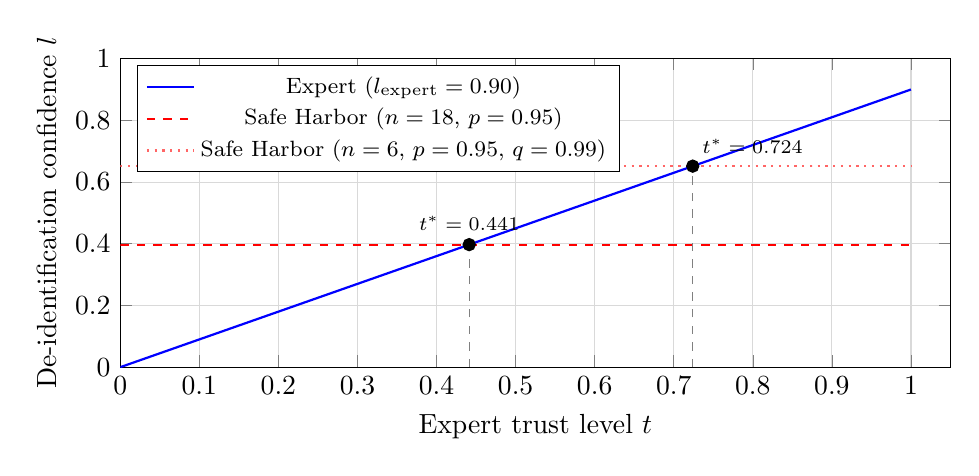
\begin{tikzpicture}
\begin{axis}[
    width=\columnwidth,
    height=5.5cm,
    xlabel={Expert trust level $t$},
    ylabel={De-identification confidence $l$},
    xmin=0, xmax=1.05,
    ymin=0, ymax=1.0,
    legend style={at={(0.02,0.98)}, anchor=north west, font=\footnotesize},
    grid=major,
    grid style={gray!30},
    every axis plot/.append style={thick},
]

% Expert Determination: l_ED = t * 0.90
\addplot[blue, domain=0:1, samples=50] {x * 0.90};
\addlegendentry{Expert ($l_{\text{expert}} = 0.90$)}

% Safe Harbor (all 18 present): 0.95^18 = 0.3972
\addplot[red, dashed, domain=0:1] {0.3972};
\addlegendentry{Safe Harbor ($n=18$, $p=0.95$)}

% Safe Harbor (Synthea, 6 present): 0.6516
\addplot[red!60, dotted, domain=0:1] {0.6516};
\addlegendentry{Safe Harbor ($n=6$, $p=0.95$, $q=0.99$)}

% Crossover markers
\addplot[only marks, mark=*, mark size=2pt, black, fill=black]
    coordinates {(0.4413, 0.3972)};
\addplot[only marks, mark=*, mark size=2pt, black, fill=black]
    coordinates {(0.7240, 0.6516)};

% Threshold annotations
\draw[gray, thin, dashed] (axis cs:0.4413,0) -- (axis cs:0.4413,0.3972);
\draw[gray, thin, dashed] (axis cs:0.7240,0) -- (axis cs:0.7240,0.6516);

\node[font=\scriptsize, anchor=south] at (axis cs:0.4413,0.41) {$t^* = 0.441$};
\node[font=\scriptsize, anchor=south west] at (axis cs:0.7240,0.66) {$t^* = 0.724$};

\end{axis}
\end{tikzpicture}
\caption{Expert Determination vs.\ Safe Harbor de-identification confidence across trust levels. Crossover points (Theorem~2): Expert exceeds Safe Harbor when $t > p^{n} q^{18-n}/l_{\text{expert}}$. With all 18 identifiers removed at $p = 0.95$, an expert trusted above $t^* = 0.441$ yields higher confidence than Safe Harbor; for the Synthea profile ($n = 6$, $q = 0.99$) the threshold is $t^* = 0.724$.}
\label{fig:trust_crossover}
\end{figure}


\subsection{Operator H3: Minimum Necessary Rule}

HIPAA \S164.502(b) requires limiting PHI to the minimum necessary. We model three conditions:

\textbf{Definition 4.} $\text{MinNec}(\omega_{\text{role}}, \omega_{\text{purpose}}, \omega_{\text{scope}}) = J_\sqcap(\omega_{\text{role}}, \omega_{\text{purpose}}, \omega_{\text{scope}})$

\textbf{Theorem 3 (Weakest Link).} If any component has $l = 0$, then $l_{\text{MN}} = 0$.

\subsection{Operator H4: BAA Trust Chain}

HIPAA \S164.502(e) governs Business Associate Agreements. BAA chains arise naturally: Covered Entity $\to$ BA $\to$ Sub-BA.

\textbf{Definition 5.} $\text{BAAChain}(\omega_S, [(\tau_1, \pi_1), \ldots]) = \text{Prop}_n \circ \cdots \circ \text{Prop}_1(\omega_S)$, where each $\text{Prop}_i$ applies Compliance Propagation.

\textbf{Theorem 4 (Multiplicative Decay).} $l_{D_n} = l_S \cdot \prod_{i=1}^{n} (t_i \cdot p_i)$.

\begin{table}[t]
\centering
\caption{BAA chain degradation ($l_S = 0.95$, $t = 0.90$, $p = 0.95$). Theory matches empirical results exactly.}
\label{tab:baa_decay}
\begin{tabular}{@{}rcr@{}}
\toprule
Depth $n$ & $l_{D_n}$ & Degradation \\
\midrule
0 & 0.950 & 0.0\% \\
1 & 0.812 & 14.5\% \\
2 & 0.694 & 26.9\% \\
3 & 0.594 & 37.5\% \\
\bottomrule
\end{tabular}
\end{table}

\subsection{Dual-Regime Composition}

\textbf{Definition 6.} $\text{DualRegime}(\omega_{\text{HIPAA}}, \omega_{\text{GDPR}}) = J_\sqcap(\omega_{\text{HIPAA}}, \omega_{\text{GDPR}})$

\textbf{Theorem 5.} (a)~$l_{\text{dual}} \leq \min(l_{\text{HIPAA}}, l_{\text{GDPR}})$. (b)~Commutative. (c)~Vacuous opinion in either regime forces $l_{\text{dual}} = 0$.

% ===================================================================
% TABLE: Dual-Regime Composition Scenarios (from E3 results)
% Shows HIPAA, GDPR, and composite opinions for three data states
% ===================================================================

\begin{table}[t]
\centering
\caption{Dual-regime composition across three data scenarios. Composite compliance (Theorem~5) is strictly lower than either individual regime.}
\label{tab:dual_regime}
\begin{tabular}{@{}lccc@{}}
\toprule
& HIPAA $l$ & GDPR $l$ & Dual $l$ \\
\midrule
Raw patient data & $8.44 \times 10^{-9}$ & 0.009 & $7.60 \times 10^{-11}$ \\
Safe Harbor de-identified & 0.652 & 0.450 & 0.293 \\
Expert de-identified & 0.765 & 0.550 & 0.421 \\
\bottomrule
\end{tabular}
\end{table}


%===================================================================
\section{Privacy-Preserving Compliance Assessment}
%===================================================================

Consider a hospital where multiple departments must compute aggregate HIPAA compliance without revealing individual scores. The Jurisdictional Meet is the aggregation operator. The challenge is computing $J_\sqcap$ without any party learning another's opinion.

Since $J_\sqcap$ requires only additions and multiplications (Eq.~\ref{eq:jmeet}), it is directly computable under the CKKS scheme~\cite{cheon2017ckks}. We encrypt each opinion component as a CKKS scalar and compute:
\begin{align}
\text{Enc}(l_\sqcap) &= \text{Enc}(l_1) \otimes \text{Enc}(l_2) \\
\text{Enc}(v_\sqcap) &= \text{Enc}(v_1) \oplus \text{Enc}(v_2) \ominus (\text{Enc}(v_1) \otimes \text{Enc}(v_2))
\end{align}

After decryption, normalization enforces $l + v + u = 1$. In our experiments, the raw constraint violation before normalization was $6.70 \times 10^{-13}$, near machine epsilon, so normalization is a safeguard rather than a correction.

% ===================================================================
% TABLE: HE Benchmark Results (from EH3 results)
% Accuracy, latency, and chain depth stability
% ===================================================================

\begin{table}[t]
\centering
\caption{CKKS homomorphic encryption benchmark for Jurisdictional Meet. Accuracy measured as max absolute error vs.\ plaintext across 1000 random opinion pairs. Latency excludes one-time key generation (204\,ms).}
\label{tab:he_benchmarks}
\begin{tabular}{@{}lcc@{}}
\toprule
Metric & Value & Threshold \\
\midrule
\multicolumn{3}{@{}l}{\textit{Accuracy (depth 1, $n=1000$)}} \\
\quad Mean error ($l$) & $3.24 \times 10^{-8}$ & $< 0.001$ \\
\quad Max error ($l$) & $1.19 \times 10^{-7}$ & $< 0.001$ \\
\quad Constraint violation (raw) & $6.70 \times 10^{-13}$ & $< 10^{-4}$ \\
\quad Constraint violation (normalized) & $2.22 \times 10^{-16}$ & $< 10^{-4}$ \\
\midrule
\multicolumn{3}{@{}l}{\textit{Latency ($n=1000$)}} \\
\quad Encrypt (2 opinions) & 19.26\,ms (p50) & -- \\
\quad Compute ($J_\sqcap$) & 6.06\,ms (p50) & -- \\
\quad Decrypt + normalize & 1.93\,ms (p50) & -- \\
\quad Total & 27.34\,ms (p50) & $< 100$\,ms \\
\quad Plaintext baseline & 0.002\,ms (p50) & -- \\
\quad Overhead factor & $15{,}186\times$ & -- \\
\midrule
\multicolumn{3}{@{}l}{\textit{Chain depth ($n=100$ per depth)}} \\
\quad Depth 1 & $1.07 \times 10^{-7}$ max & $< 0.001$ \\
\quad Depth 2 & $4.27 \times 10^{-7}$ max & $< 0.001$ \\
\quad Depth 3 & $3.97 \times 10^{-6}$ max & $< 0.01$ \\
\quad Depth 4 & $1.95 \times 10^{-6}$ max & $< 0.01$ \\
\quad Depth 5 & $2.65 \times 10^{-6}$ max & $< 0.01$ \\
\bottomrule
\end{tabular}
\end{table}


The overhead is substantial: $15{,}186\times$ compared to plaintext computation. However, the absolute latency of 27\,ms per operation is acceptable for compliance assessment, which is not a real-time control task. We report this overhead prominently because honest characterization of limitations strengthens rather than weakens a feasibility claim.

% ===================================================================
% FIGURE: HE Chain Depth Accuracy (from EH3 depth study)
% Shows max error remains stable across depths 1-5
% Requires: \usepackage{pgfplots} in preamble
% ===================================================================

\begin{figure}[t]
\centering
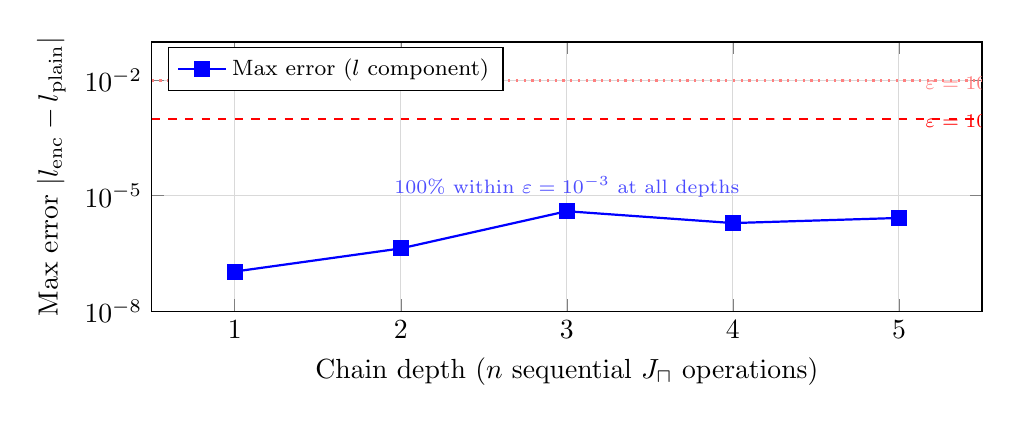
\begin{tikzpicture}
\begin{axis}[
    width=\columnwidth,
    height=5cm,
    xlabel={Chain depth ($n$ sequential $J_\sqcap$ operations)},
    ylabel={Max error $|l_{\text{enc}} - l_{\text{plain}}|$},
    ymode=log,
    xmin=0.5, xmax=5.5,
    ymin=1e-8, ymax=1e-1,
    xtick={1,2,3,4,5},
    legend style={at={(0.02,0.98)}, anchor=north west, font=\footnotesize},
    grid=major,
    grid style={gray!30},
    every axis plot/.append style={thick},
]

% Max error per depth
\addplot[blue, mark=square*, mark size=2.5pt]
    coordinates {
        (1, 1.07e-07)
        (2, 4.27e-07)
        (3, 3.97e-06)
        (4, 1.95e-06)
        (5, 2.65e-06)
    };
\addlegendentry{Max error ($l$ component)}

% Threshold lines
\addplot[red, dashed, domain=0.5:5.5] {0.001};
\addplot[red!50, dotted, domain=0.5:5.5] {0.01};

\node[font=\scriptsize, red, anchor=west] at (axis cs:5.1, 0.001) {$\varepsilon = 10^{-3}$};
\node[font=\scriptsize, red!50, anchor=west] at (axis cs:5.1, 0.01) {$\varepsilon = 10^{-2}$};

% Annotation
\node[font=\scriptsize, anchor=south, text=blue!70] at (axis cs:3, 5e-6)
    {100\% within $\varepsilon = 10^{-3}$ at all depths};

\end{axis}
\end{tikzpicture}
\caption{CKKS encrypted $J_\sqcap$ accuracy across chain depths. Max error over 100 trials per depth remains below $\varepsilon = 10^{-3}$ through depth 5, demonstrating that noise accumulation is well-managed by automatic parameter scaling. Overhead: $15{,}186\times$ vs.\ plaintext (27\,ms vs.\ 0.002\,ms).}
\label{fig:he_depth}
\end{figure}


%===================================================================
\section{Evaluation}
%===================================================================

\subsection{Operator Property Verification}

We verified Theorems~1 through 5 using property-based testing with the Hypothesis framework. For each operator, 10,000 random compliance opinions were generated across 33 distinct properties. All 33 tests pass with zero counterexamples. The constraint $l + v + u = 1$ holds within $\varepsilon < 10^{-9}$ for every composition.

\subsection{Clinical Compliance Pipeline}

We evaluated the operators on 100 synthetic patient bundles generated by Synthea~\cite{walonoski2018synthea}, containing FHIR R4 resources across 32 types.

\textbf{PHI Classification.} All 100 patients contain exactly 6 HIPAA identifier categories (names, addresses, dates, phone numbers, SSNs, other identifiers). The resulting $l_{\text{PHI}} = 8.44 \times 10^{-9}$, confirming that raw patient data is correctly classified as PHI. The uniform identifier profile across Synthea patients is an honest limitation of the synthetic data source, not of the algebra.

\textbf{Progressive De-identification.} Fig.~\ref{fig:progressive_deident} shows $l_{\text{PHI}}$ recovery as identifiers are removed one by one. Each removal increases $l$ by approximately $19\times$ (the ratio $0.95/0.05$). After removing all 6 present identifiers, $l$ recovers to $0.397 = 0.95^{18}$, matching theory exactly.

% ===================================================================
% FIGURE: Progressive De-identification Recovery (from E2 results)
% Shows l_PHI recovery as identifiers are removed one by one
% Requires: \usepackage{pgfplots} in preamble
% ===================================================================

\begin{figure}[t]
\centering
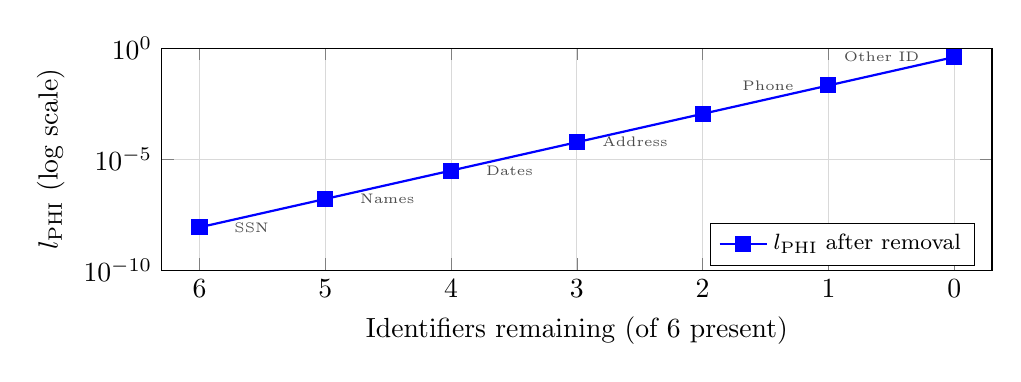
\begin{tikzpicture}
\begin{axis}[
    width=\columnwidth,
    height=4.4cm,
    xlabel={Identifiers remaining (of 6 present)},
    ylabel={$l_{\text{PHI}}$ (log scale)},
    ymode=log,
    xmin=-0.3, xmax=6.3,
    ymin=1e-10, ymax=1,
    xtick={0,1,2,3,4,5,6},
    xticklabels={0,1,2,3,4,5,6},
    x dir=reverse,
    legend style={at={(0.98,0.02)}, anchor=south east, font=\footnotesize},
    grid=major,
    grid style={gray!30},
    every axis plot/.append style={thick},
    nodes near coords style={font=\tiny, anchor=south west},
]

% Progressive de-identification data points
\addplot[blue, mark=square*, mark size=2.5pt]
    coordinates {
        (6, 8.443126e-09)
        (5, 1.604194e-07)
        (4, 3.047969e-06)
        (3, 5.791140e-05)
        (2, 1.100317e-03)
        (1, 2.090602e-02)
        (0, 3.972143e-01)
    };
\addlegendentry{$l_{\text{PHI}}$ after removal}

% Annotations for key steps
\node[font=\tiny, anchor=west, text=black!70] at (axis cs:5.8, 8.4e-09) {SSN};
\node[font=\tiny, anchor=west, text=black!70] at (axis cs:4.8, 1.6e-07) {Names};
\node[font=\tiny, anchor=west, text=black!70] at (axis cs:3.8, 3.0e-06) {Dates};
\node[font=\tiny, anchor=east, text=black!70] at (axis cs:2.2, 5.8e-05) {Address};
\node[font=\tiny, anchor=east, text=black!70] at (axis cs:1.2, 2.1e-02) {Phone};
\node[font=\tiny, anchor=east, text=black!70] at (axis cs:0.2, 3.97e-01) {Other ID};

\end{axis}
\end{tikzpicture}
\caption{Progressive de-identification of a Synthea patient record: each removal raises $l_{\text{PHI}}$ by about $19\times$ (the ratio $0.95/0.05$), from $8.44 \times 10^{-9}$ with 6 identifiers to $0.397 = 0.95^{18}$ after full removal; theory-validated at every step.}
\label{fig:progressive_deident}
\end{figure}


\textbf{De-identification Comparison.} Safe Harbor yields $l_{\text{SH}} = 0.652$ ($= 0.95^6 \cdot 0.99^{12}$). Expert Determination at trust $t = 0.85$ yields $l_{\text{ED}} = 0.765$. Expert exceeds Safe Harbor for all 100 patients, with trust threshold $t^* = 0.724$, validating Theorem~2.

\textbf{Cross-Resource Profiles.} Different FHIR resource types contain different identifier subsets (Table~\ref{tab:cross_resource}), producing $l_{\text{PHI}}$ values spanning eight orders of magnitude, from $1.10 \times 10^{-3}$ (Condition, 2~identifiers) to $2.34 \times 10^{-11}$ (Claim, 8~identifiers).

% ===================================================================
% TABLE: Cross-Resource-Type PHI Profiles (from E5 results)
% Shows how different FHIR resource types have different identifier counts
% and correspondingly different PHI classification confidence
% ===================================================================

\begin{table}[t]
\centering
\caption{PHI classification across FHIR R4 resource types. Resources with more HIPAA identifiers have exponentially lower compliance confidence. All predictions match theory.}
\label{tab:cross_resource}
\begin{tabular}{@{}lccc@{}}
\toprule
Resource Type & $n_{\text{IDs}}$ & $l_{\text{PHI}}$ & $v_{\text{PHI}}$ \\
\midrule
Condition           & 2 & $1.10 \times 10^{-3}$ & 0.993 \\
Observation         & 3 & $5.79 \times 10^{-5}$ & 0.999 \\
MedicationRequest   & 3 & $5.79 \times 10^{-5}$ & 0.999 \\
DiagnosticReport    & 5 & $1.60 \times 10^{-7}$ & $\approx 1.0$ \\
ImagingStudy        & 5 & $1.60 \times 10^{-7}$ & $\approx 1.0$ \\
Patient             & 6 & $8.44 \times 10^{-9}$ & $\approx 1.0$ \\
Claim               & 8 & $2.34 \times 10^{-11}$ & $\approx 1.0$ \\
\bottomrule
\end{tabular}
\end{table}


\subsection{Temporal Decay of Compliance Assessments}

HIPAA requires ongoing compliance through periodic review
(45~CFR~164.530(i))~\cite{hipaa_security}. Binary tools provide no mechanism
to trigger reassessment: a two-year-old PASS is indistinguishable from
today's PASS. The compliance algebra models assessment staleness through
opinion decay~\cite{josang2016subjective}, where evidence migrates from
belief and disbelief into uncertainty over time.

Table~\ref{tab:temporal_decay} shows a strong initial assessment
($l = 0.900$, $v = 0.050$, $u = 0.050$) decaying with an exponential half-life
of one year. After two years, lawfulness confidence drops to 0.225 while
uncertainty grows to 0.762. The assessment has not become a known
violation ($v$ remains low at 0.013); rather, the evidence has become
stale. The projected probability $P(\omega)$ declines from 0.925 to 0.606,
crossing below a hypothetical reassessment threshold of 0.70 between
one and two years.

\begin{table}[t]
\centering
\caption{Temporal decay of a HIPAA compliance assessment ($l_0 = 0.90$, half-life = 1 year). Binary tools report PASS at all times.}
\label{tab:temporal_decay}
\begin{tabular}{@{}lcccc@{}}
\toprule
Period & $l$ & $v$ & $u$ & $P(\omega)$ \\
\midrule
Day 0 (fresh)  & 0.900 & 0.050 & 0.050 & 0.925 \\
6 months       & 0.639 & 0.036 & 0.325 & 0.802 \\
1 year         & 0.450 & 0.025 & 0.525 & 0.713 \\
2 years        & 0.225 & 0.013 & 0.762 & 0.606 \\
3 years        & 0.113 & 0.006 & 0.881 & 0.553 \\
\bottomrule
\end{tabular}
\end{table}

This behavior directly supports the regulatory intent of 45~CFR~164.530(i):
organizations must ``review and modify'' security policies ``as needed.'' The
algebra provides a principled trigger for this review by quantifying when
accumulated uncertainty exceeds an acceptable threshold. The distinction between
$u$~growing (stale evidence) and $v$~growing (new violation evidence) informs
the appropriate response: reassess versus investigate.

\subsection{End-to-End Clinical Workflow}

We trace a complete compliance lifecycle for a synthetic patient to
demonstrate how the operators compose in practice.

\textbf{Step 1: PHI Classification.} A Synthea patient record contains
six HIPAA identifier categories (names, addresses, dates, phone numbers,
SSN, and a facility identifier). PHI Classification produces
$\omega_{\text{PHI}} = (8.44 \times 10^{-9},\; 0.9999,\; 7.76 \times 10^{-7},\; 3.81 \times 10^{-6})$,
confirming the record as PHI with near-certainty ($P = 8.45 \times 10^{-9}$).
A compliance officer seeing this opinion knows the data requires protection
under the Privacy Rule before any sharing.

\textbf{Step 2: De-identification.} The hospital applies Safe Harbor
de-identification, removing the six present identifiers with per-identifier
removal confidence $p = 0.95$. The Safe Harbor assessment yields
$l_{\text{SH}} = 0.652$. An available expert ($l_{\text{expert}} = 0.90$,
trust $t = 0.85$) produces $l_{\text{ED}} = 0.765$. The expert method
provides 17\% higher confidence, quantifying the value of Expert
Determination over mechanical Safe Harbor removal.

\textbf{Step 3: BAA Chain.} The de-identified data is shared with a
laboratory partner (BA) for secondary analysis. Using the hospital's
post-de-identification compliance ($l = 0.652$) as the source, a single
BAA link with safeguard trust $t = 0.90$ and purpose compatibility
$p = 0.95$ yields $l_{D_1} = 0.557$, a 14.5\% degradation. If the
laboratory subcontracts to a cloud analytics provider (sub-BA) with
weaker safeguards ($t = 0.75$, $p = 0.85$), the chain degrades further
to $l_{D_2} = 0.355$.

\textbf{Step 4: Dual-Regime.} The laboratory's EU affiliate requests
access for a joint clinical trial. GDPR compliance is assessed at
$\omega_{\text{GDPR}} = (0.450, 0.250, 0.300, 0.30)$, reflecting the
additional requirements of lawful basis and data minimization. The
dual-regime composition yields $l_{\text{dual}} = 0.293$, a 55\%
reduction from the HIPAA assessment alone. The composite opinion
$(0.293, 0.475, 0.232)$ reveals that violation risk ($v = 0.475$)
exceeds lawfulness confidence, signaling that additional safeguards
or a more favorable GDPR assessment are needed before cross-border
transfer proceeds.

This four-step workflow is impossible with binary compliance tools, which
can only report PASS or FAIL at each stage. The algebra preserves the
full epistemic state through every transformation, enabling
risk-proportionate decision-making at each step.

\subsection{Comparison with Binary Approaches}

Table~\ref{tab:binary_scenarios} presents five scenarios where binary assessment collapses distinct epistemic states. The strongest distinction is Scenario~2 (new vendor): binary tools assign the same FAIL to complete ignorance ($u = 1.0$) and known violation ($v = 1.0$), though the projected probabilities differ ($P = 0.5$ vs.\ $P = 0.0$) and the appropriate responses (gather evidence vs.\ block access) are entirely different.

% ===================================================================
% TABLE: Binary vs Algebra Comparison (from EH4 results)
% Five clinically motivated scenarios
% ===================================================================

\begin{table*}[t]
\centering
\caption{Five clinically motivated scenarios comparing binary HIPAA compliance assessment with the proposed algebra. Each scenario demonstrates an epistemic state that binary tools collapse. All algebra values computed using the implemented operators.}
\label{tab:binary_scenarios}
\begin{tabular}{@{}p{3.8cm}p{2.8cm}p{3.2cm}p{5.5cm}@{}}
\toprule
Scenario & Binary Result & Algebra $(l, v, u)$ & Distinction \\
\midrule
Conflicting audit evidence (two auditors disagree)
  & 50\% / Inconclusive
  & $(0.085, 0.810, 0.105)$
  & High $v$ with low $u$ reveals active conflict requiring investigation, not more data. \\[4pt]
New vendor (no compliance history)
  & FAIL
  & $(0.000, 0.000, 1.000)$
  & Ignorance ($u\!=\!1$) is distinct from violation ($v\!=\!1$). Response: gather evidence, not block. \\[4pt]
BAA chain (hospital, lab, billing)
  & FAIL (any weak link)
  & $(0.176, 0.502, 0.322)$
  & Quantifies 80.9\% total degradation. Billing link identified as primary risk driver. \\[4pt]
Stale assessment (2 years old)
  & PASS (no expiration)
  & $(0.225, 0.013, 0.762)$
  & $l$ decays 0.900\,$\to$\,0.225, $u$ grows 0.050\,$\to$\,0.762. Triggers reassessment. \\[4pt]
HIPAA + GDPR (uncertain vs.\ violated)
  & FAIL (both cases)
  & $(0.352, 0.184, 0.464)$
  & Uncertain GDPR ($u\!=\!0.46$) vs.\ violated GDPR ($v\!=\!0.90$): proceed with monitoring vs.\ halt. \\
\bottomrule
\end{tabular}
\end{table*}


\subsection{Independence Assumptions}

PHI Classification assumes independent identifier presence. Positive correlation (identifiers co-occur) means true risk exceeds our estimate: the bias is non-conservative. Minimum Necessary assumes independent role, purpose, and scope assessment; since certain roles imply purpose, independence may overstate uncertainty: the bias is conservative. We document all bias directions to enable informed interpretation.

%===================================================================
\section{Discussion}
%===================================================================

The HIPAA operators extend the GDPR compliance algebra implemented in \texttt{jsonld-ex}~\cite{syed2026jsonldex}, which defines five operators on the same primitives; the HIPAA operators add HIPAA-specific semantic mappings. The dual-regime composition confirms that both algebras compose via Jurisdictional Meet, validating regulation-agnostic design.

Limitations include: (1)~the HIPAA-to-algebra mapping involves interpretive choices that compliance experts may dispute; (2)~all base rates are illustrative, not empirically calibrated against enforcement data; (3)~the HE proof-of-concept demonstrates feasibility but not deployment readiness, with $15{,}186\times$ overhead; (4)~Synthea generates uniform patient demographics, limiting variance in the empirical evaluation.

The algebra enables workflows that binary tools cannot support. A compliance officer can distinguish ``probably compliant'' ($l$ high, $u$ low) from ``uncertain'' ($u$ high) from ``conflicting evidence'' ($l$ and $v$ both elevated). These distinctions support different response strategies. The BAA chain operator quantifies compliance degradation through business associate relationships, providing a basis for supply chain risk management consistent with \S164.502(e)~\cite{hipaa_security}.

%===================================================================
\section{Conclusion}
%===================================================================

We presented a HIPAA compliance algebra that models healthcare privacy compliance as uncertain epistemic states. The algebra provides four operators grounded in specific HIPAA provisions, with properties verified through property-based testing. We demonstrated dual-regime GDPR and HIPAA composition and presented a proof-of-concept for privacy-preserving compliance aggregation using homomorphic encryption that stays within $1.19 \times 10^{-7}$ of plaintext for a single operation and within $4.0 \times 10^{-6}$ across chain depths up to five.

Future work includes empirical calibration of base rates against enforcement data, extension to additional healthcare regulations, and collaboration with legal scholars to validate the HIPAA-to-algebra mapping. The implementation is available as part of \texttt{jsonld-ex} on PyPI.

\balance
\bibliographystyle{IEEEtran}
\bibliography{refs}

\end{document}
